\section{08.01.24 : Funktor pochodny }

Przypominając wykład sprzed tygodnia, prawy funktor pochodny $RF$ powstaje przez złożenie czerwonych strzałek:

\begin{center}\begin{tikzcd}
  K^+(I_\mathbf{A})\arrow[r]\arrow[dr, yshift=1mm, "\iota"]\arrow[rr, bend left=20, yshift=2mm, red] & K^+(\mathbf{A})\arrow[r, "K(F)"]\arrow[d] & K^+(\mathbf{B})\arrow[d] \arrow[d, red, bend left=20, xshift=2mm]\\ 
                                                            & D^+(\mathbf{A})\arrow[ul, "\iota^{-1}", yshift=-1mm]\arrow[r, red, "RF" below] \arrow[ul, red, bend left=20, yshift=-2mm, xshift=-2mm] & D^+(\mathbf{B})
\end{tikzcd}\end{center}

%\begin{definition}
%  Dla dowolnego $A\in\ob\mathbf{A}$ definiujemy
%  $$R^iF(A):=H^i(RF(A[0]))$$
%\end{definition}
%
%\begin{fact}
%  Jeśli $F$ jest lewo dokładny, i $0\to A\to B\to C\to 0$ jest dokładny w $\mathbf{A}$, to również
%  \begin{center}\begin{tikzcd}
%    0\arrow[r] & F(A)\arrow[r] & F(B)\arrow[r] & F(C)\arrow[r] R^1F(A)\arrow[r] R^1F(B)\arrow[r] & R^1F(C)\arrow[r] & R^2F(A)\arrow[r] & ...
%    \end{tikzcd}\end{center}
%    jest ciągiem dokładnym.
%\end{fact}

\subsection{Własności funktora pochodnego}

\begin{fact}
  $$Ext_\mathbf{A}^i(A,-)=R^iHom(A, -)$$
\end{fact}

\begin{proof}
  Policzmy $(R^iHom(A, -))(B)$ dla dowolnego $B\in \mathbf{A}$. Mamy rezolwentę injektywną
  $$B\to I^0\to I^1\to I^2\to ...$$
  dostajemy wówczas
  \begin{center}\begin{tikzcd}
    ...\arrow[r] & 0\arrow[r] & Hom(A, I^0)\arrow[r] & Hom(A, I^1)\arrow[r] & Hom(A, I^2)
  \end{tikzcd}\end{center}
  Szukana grupa (obiekt) to 
  $$\ker d:\frac{Hom(A, I^i)\to Hom(A, I^{i+1})}{\img d:Hom(A, I^{i+1})\to Hom(A, I^i)}/$$
  Dowolna strzałka $Hom(A, I^i)\ni f:A\to I^i$ jest w $\ker d$ $\iff$ odwzorowanie
  \begin{center}\begin{tikzcd}
    ...\arrow[r] & 0\arrow[r]\arrow[d, "0"] & A\arrow[r]\arrow[d, "f"] & 0\arrow[r]\arrow[d, "0"] & 0\arrow[r]\arrow[d, "0"] & ...\\
    ...\arrow[r] & I^{i-1} \arrow[r] & I^i\arrow[r] & I^{i+1}\arrow[r] & I^{i+2}\arrow[r] & ...
  \end{tikzcd}\end{center}
  jest morfizmem kompleksów
  $$\ker d:\underbrace{Hom(A, I^i)}_{=Hom_{Kom\mathbf{A}}(A[i], I^*)}\to Hom(A, I^{i+1})$$

  Taka sama strzałka $f:A\to I^i$ jest w obrazie $\img d$ $\iff$ odwzorowanie kompleksów
  \begin{center}\begin{tikzcd}
    0\arrow[r]\arrow[d] & A\arrow[r]\arrow[d, "f"]\arrow[dl, green, "h"] & 0\arrow[d]\\ 
    I^{i-1}\arrow[r] & I^i\arrow[r] & I^{i+1}
  \end{tikzcd}\end{center}
  jest homotopijne z zerem.

  Zatem dostajemy
  $$H^i(Hom(A, I^*))=Hom_{K^+(\mathbf{A})}(A[i], I^*)$$
  ale ponieważ $I^*$ jest injektywny, to
  $$Hom_{K^+(\mathbf{A})}(A[i], I^*)=Hom_{D^+(\mathbf{A})}(A[i], I^*)$$
  ale przecież w  $D^+\mathbf{A}$ mamy $I^*\cong B[0]$, więc
  $$Hom_{D^+\mathbf{A}}(A[i], I^*)=Hom_{D^+\mathbf{A}}(A[i], B[0])=Ext^i_{\mathbf{A}}(A, B).$$
\end{proof}

\begin{fact}
  \begin{enumerate}
    \item $RF$ jest dokładny.
    \item $\exists$ naturalne przekształcenie $\epsilon_F:Q_B\circ K(F)\implies RF\circ Q_A$
    \item Jeśli $G:D^+\mathbf{A}\to D^+\mathbf{B}$ jest dokładny i dopuszcza naturalne przekształcenie $\epsilon_G:Q_B\circ K(F)\implies G\circ Q_A$ analogiczne jak wyżej, to istnieje naturalne przekształcenie $\eta:RF\to G$, które zamyka diagram
      \begin{center}\begin{tikzcd}
        & RF\circ Q_A\arrow[dd, "\eta"]\\
        Q_B\circ K(F)\arrow[ur, "\epsilon_F"]\arrow[dr, "\epsilon_G"]\\ 
        & G\circ Q_A
      \end{tikzcd}\end{center}
  \end{enumerate}
\end{fact}

\begin{proof}
  \begin{enumerate}
    \item Mając dany trójkąt wyróżniony \begin{tikzcd} A^*\arrow[r, "f"] & B^*\arrow[r] & C(f)\arrow[r] & A^*[1] \end{tikzcd} produkujemy stożek w sposób funktorialny
      \begin{center}\begin{tikzcd}
        F(A^*)\arrow[r, "F(f)"] & F(B^*)\arrow[r] & F(C(f))\arrow[r, "="] & C(F(f))
      \end{tikzcd}\end{center}

      Stąd $K(F)$ i $Q_B$ są dokładne. Ponieważ $RF=Q_B\circ K(F)\circ \iota^{-1}$, to wystarczy pokazać, że $\iota^{-1}$ jest dokładna.

      Bierzemy więc trójkąt wyróżniony w $D^+\mathbf{A}$, zaznaczony na zielono. Naszym celem będzie pokazać, że druga od góry linijka jest trójkątem wyróżninym
      \begin{center}\begin{tikzcd}
        \iota^{-1}A\arrow[r, "g"]\arrow[d, "="] & \iota^{-1} B\arrow[r]\arrow[d, "="] & C(g) \arrow[r] & \iota^{i-1}A[1]\arrow[d, "="] & \Delta\text{ w }K^+(I_\mathbf{A})\\

        \iota^{-1}A\arrow[r, "g"]\arrow[d, "\cong"] &\iota^{-1} B\arrow[r]\arrow[d, "\cong"] & \iota^{-1}C\arrow[r]\arrow[d, "\cong"] & \iota^{-1}A[1]\arrow[d, "\cong"] & \text{trójkąt w }K^+(I_\mathbf{A})\\
        \color{green}A\arrow[r, green] \arrow[d, "\cong"] &\color{green} B\arrow[r, green]\arrow[d, "\cong"] & \color{green} C\arrow[r, green] \arrow[d, "\cong"] & \color{green} A[1]\arrow[d, "\cong"] & \text{wyjściowy }\Delta\\ 
        A'\arrow[r]\arrow[uuu, bend left=20, orange] & B'\arrow[r]\arrow[uuu, bend left=20, orange] & C(f)\arrow[r]\arrow[uuu, dashed, orange, bend left=20, "\exists\phi" left] & A'[1]\arrow[uuu, bend right=20, orange] & \Delta\text{ w }Kom^+(\mathbf{A})
      \end{tikzcd}\end{center}
      pomarańczowa strzałka istnieje, ponieważ pomarańczowe strzałki to izomorfizmy między wyrazami trójkątów wyróżnionych -> musi się więc domknąć do pełnego odwzorowania między tymi trójkątami. Pokażemy teraż, że $\phi:C(f)\to C(g)$ jest qis. Rozważamy ciągi dokładne trójkątów:
      \begin{center}\begin{tikzcd}
        H^i(\iota^{-1}A)\arrow[r] & Hom^i(\iota^{-1}B)\arrow[r] & H^i(C(g))\arrow[r] & H^{i+1}(\iota^{-1}A)\arrow[r] & Hom^{i+1}(\iota^{-1}B)\\ 
        H^i(A')\arrow[u, "\cong"]\arrow[r] & H^i(B')\arrow[u, "\cong"]\arrow[r] & H^i(C(f))\arrow[u,dashed]\arrow[r] & H^{i+1}(A')\arrow[u, "\cong"]\arrow[r] & H^{i+1}(B')\arrow[u, "\cong"]
      \end{tikzcd}\end{center}
      z lematu o $5$ izomorfizmach wiemy, że strzałka z $H^i(C(f))$ jest izomorfizmem, czyli w rzeczy samej, $\phi$ jest qis.

      Mamy więc z tego odwzorowanie trójkąta z drugiej linii do trójkąta z 1 linii i to odwzorowanie jest izomorfizmem w $D^+(\mathbf{A})$. Ponieważ 1 i 2 linia składają się z obiektów injektywnych, to izomorfizm ten realizuje się w $K^+(\mathbf{A})$.

    \item Pytamy o istnienie strzałki $\epsilon_F$ na diagramie
      \begin{center}\begin{tikzcd}[column sep=large, row sep=large]
        K^+\mathbf{A}\arrow[r, "K(F)"]\arrow[d, "Q_A" left] & K^+\mathbf{B}\arrow[d, "Q_B"]\arrow[dl, "\varepsilon_F" above left, bend right=30, Rightarrow, xshift=3mm, yshift=-5mm, end anchor = {[xshift=3mm, yshift=2mm]north east}]\\ 
        D^+\mathbf{A}\arrow[r, "RF" below] & D^+\mathbf{B}
      \end{tikzcd}\end{center}
      
      Rysujemy diagram
      \begin{center}\begin{tikzcd}
        & A^*\arrow[r, "KF"] \arrow[d, "Q_A"] & F(A^*)\arrow[d, "Q_B"]\\ 
        & A^*\arrow[dl, "\mu(A^*)" above left]\arrow[d, "RF"] & \arrow[ddl, bend left=40, "F(\mu(A^*))"] F(A^*)\\ 
        I^* & RF(A^*)\arrow[d, "\cong" left]\\ 
        \iota\iota^{-1}(A^*)\arrow[u, phantom, sloped, "="]& F(I^*)
      \end{tikzcd}\end{center}
      gdzie \begin{tikzcd}\mu:ID_{D^+\mathbf{A}}\arrow[r, Rightarrow] &\iota\iota^{-1}\end{tikzcd} jest naturalnym przekształceniem. Szukany $\epsilon_F=F\mu$.
    \item Diagram wygląda następująco
      \begin{center}\begin{tikzcd}
        K^+\mathbf{A}\arrow[d] \arrow[r, "K(F)"]
        \arrow[dr, blue, to path={ -- ([yshift=1mm]\tikztostart.north)  -| ([yshift=1cm]\tikztotarget.east) -- (\tikztotarget.east)}, rounded corners] 
        \arrow[dr, blue, to path={ -- ([xshift=-1mm]\tikztostart.west)  |- ([xshift=-1.4cm, yshift=-4mm]\tikztotarget.south) -| ([yshift=-2mm]\tikztotarget.south) }, rounded corners]%-- ([xhisft=4mm]\tikztotarget.east)}] 
        & K^+\mathbf{B} \arrow[d] \arrow[d, bend left=100, start anchor={[xshift=0.5mm, yshift=-7mm]}, Rightarrow, blue, "\epsilon_G", end anchor={[xshift=-3mm, yshift=-4mm]south}] \\ 
        D^+\mathbf{A} \arrow[r, bend left=20, "RF" above]\arrow[r, bend right=20, "G" below] & D^+\mathbf{B}

        \end{tikzcd}
        \begin{tikzpicture}[overlay, remember picture]
          \draw[->, orange, dashed] (-2, -0.5)--(-2, -0.85) node [midway, left] {$\scriptstyle\eta$};
      \end{tikzpicture}\end{center}
      {\large\color{red}ZDJĘCIE}
  \end{enumerate}
\end{proof}

Jeśli $A, B$ są $R$-modułami, to $Tor(A, B)$ liczymy biorąc rezolwentę projektywną
$$...\to P_1\to P_0\to B$$ 
tensorujemy ją z $A$ i dostajemy
$$...\to A\otimes P_2\to A\otimes P_1\to A\otimes P_0\to 0$$
Wtedy kohomologie tego nowego kompleksu to tory: $H^i=Tor_i(A, B)$
  
\subsection{Obiekty $F$-acykliczne}

\begin{theorem}
  Niech $\mathbf{A},\mathbf{B}$ będą kategoriami abelowymi takimi, że w $\mathbf{A}$ jest dostatecznie dużo oniektów injektywnych $I_\mathbf{A}$. Niech 
  $$F:\mathbf{A}\to \mathbf{B}$$
  będzie addytywnym i lewo-dokładnym funktorem. Niech $I_F$ będzie klasą obiektów $F$-acyklicznych. To znaczy takich $A\in\ob\mathbf{A}$, dla których $R^iF(A)=0$ dla $i>0$. Wtenczas
  \begin{enumerate} 
    \item $I_A\subseteq I_F$
    \item jeśli $A^*\in Kom^+\mathbf{A}$ jest dokładny oraz $A^i\in I_F$, to wówczas $F(A^*)$ też jest dokładny
    \item jeśli $A\to A^*$ jest rezolwentą $F$-acykliczną, to 
      $$RF(A[0])=RF(A^*)=F(A^*)$$
      a co więcej
      $$R^iF(A)=H^i(F(A^*)).$$
  \end{enumerate}
\end{theorem}

\begin{proof}
  \begin{enumerate}
    \item Niech $I\in I_A$ i chcemy sprawdzić, że wyższe pochodne $R^iF(I)=0$. Rozważamy rezolwentę injektywną $I$:
      \begin{center}\begin{tikzcd}
        I\arrow[r] & I\arrow[r]\arrow[d, "F" right] & 0\arrow[r] & 0\arrow[r] & ... \\ 
        0\arrow[r] & F(I)\arrow[r] & 0\arrow[r] & 0 \arrow[r] & ...
      \end{tikzcd}\end{center}
      czyli $H^*$ to $0\quad F(I)=R^0F(I) \quad 0\quad 0=R^2F(I)\quad ...$.
    \item  Bez straty ogólności rozważmy
      $$0\to A^0\to A^1\to A^2\to....$$
      Niech $B^i=\img(d:A^{i-1}\to A^i)$. Z dokładności $A^*$ wynika dokładność ciągu
      $$0\to A^0\to B^1\to 0.$$
      W następnym korku możemy popatrzeć na włożenie $B^1\to A^2$, którego iloraz przez jądro jest dokładnie równe $B^2$. Kontynuując ten tok myślenia dostajemy cały zestaw ciągów dokłądnych
      $$0\to B^1\to A^1\to B^2\to 0$$
      $$0\to B^2\to A^2\to B^3\to 0$$
      $$...$$
      Czyli $B^1\cong A^0$ jest $F$-acykliczny. Z zestawu ciągów dokładnych dostajemy ciąg indukowany przez $F$
      \begin{center}\begin{tikzcd}[row sep=small]
        0\arrow[r] & FB^1\arrow[r] & FA^1\arrow[r] & FB^2\arrow[dll, rounded corners,
    to path={ -- ([xshift=2ex]\tikztostart.east)
      |- ([xshift=2ex, yshift=-3ex]\tikztostart.east)
-| ([xshift=-2ex]\tikztotarget.west)
-- (\tikztotarget)}]
        \\ 
                   & R^1F(B^1)\arrow[r] & R^1F(A^1)\arrow[r] & R^1F(B^2)\arrow[r] & R^2F(B^1)\arrow[r] & ...\\ 
                   & 0\arrow[u, phantom, sloped, "="] & 0\arrow[u,phantom,sloped,"="] & 0\arrow[u, phantom, sloped, "="] & 0\arrow[u, phantom, sloped, "="]
      \end{tikzcd}\end{center}

      Ciągi dokładne wyżej możemy połączyć w diagram
      \begin{center}\begin{tikzcd}[column sep=tiny, row sep=small]
        & & 0\arrow[dr] & & 0 & & & & 0\\ 
        & & & B^k\arrow[ur]\arrow[dr] & & & & B^{k+2}\arrow[ur]\\
        & ...\arrow[r] & A^{k-1}\arrow[ur]\arrow[rr] & & A^k\arrow[rr]\arrow[dr] & & A^{k+1}\arrow[r]\arrow[ur] & ...\\ 
        & B^{k-1}\arrow[ur] & & & & B^{k+1}\arrow[dr]\arrow[ur]\\ 
        0\arrow[ur] & & & & 0\arrow[ur] & & 0
      \end{tikzcd}\end{center}
      który po przejściu przez $F$ zmienia się w 
      \begin{center}
        %\scalebox{0.9}{
      \begin{tikzcd}[scale cd=0.8, column sep=tiny, row sep=small]
        & & 0\arrow[dr] & & R^1FB^{k-1}=0 & & 0\arrow[dr] & & R^1FB^{k+1}=0\\ 
        & & & FB^k\arrow[ur]\arrow[dr] & & & & FB^{k+2}\arrow[ur]\\
        & ...\arrow[r] & FA^{k-1}\arrow[ur]\arrow[rr] & & FA^k\arrow[rr]\arrow[dr] & & FA^{k+1}\arrow[r]\arrow[ur] & ...\\ 
        & FB^{k-1}\arrow[ur] & & & & FB^{k+1}\arrow[dr]\arrow[ur]\\ 
        0\arrow[ur] & & & & 0\arrow[ur] & & 0=R^1FB^k
    \end{tikzcd}
  %}
    \end{center}
    \item Użyjemy do tego punktu rezolwenty C-E z poprzedniego wykładu (\ref{rezolwenta C-E}).
      Odwzorowanie $A[0]\to A^*$ jest qis, czyli jest izomorfizmem w $D^+\mathbf{A}$. Czyli $RF(A[0])\cong RF(A^*)$, w szczególności $R^iF(A)\cong H^i(RF(A^*))$.

      \begin{center}
          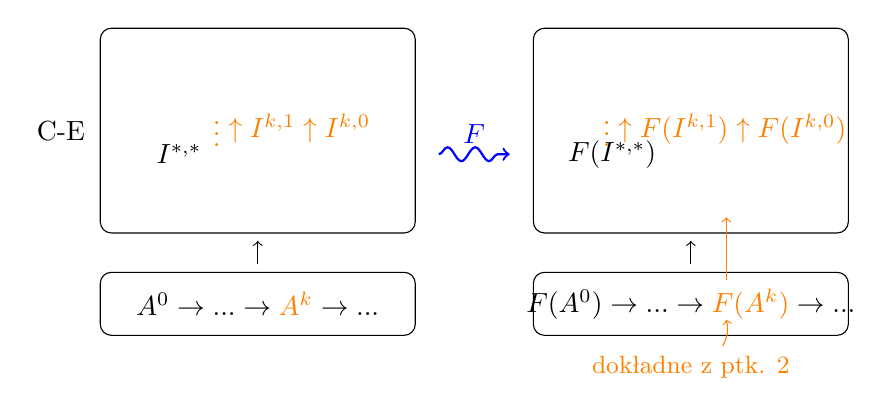
\begin{tikzpicture}
        \draw[rounded corners] (-1, 0) rectangle (3, 2.6);
        \node at (-1.5, 1.3) {C-E};
        \node at (0, 1) {$I^{*,*}$};
        
        \draw[rounded corners] (-1, -0.5) rectangle (3, -1.3);
        \draw[->] (1, -0.4)--(1, -0.1); 

        \node at (1, -0.9) {$A^0\to...\to {\color{orange}A^k}\to ...$};
        \node at (1.4, 1.3) {$\color{orange}\begin{matrix}\vdots\\\uparrow\\I^{k,1}\\\uparrow\\I^{k, 0}\end{matrix}$}; 

        \draw[blue, ->, thick, style={decorate, decoration=snake}] (3.3, 1)--(4.2, 1) node [midway, above] {$F$};


        \draw[rounded corners] (4.5, 0) rectangle (8.5, 2.6);
        \node at (5.5, 1) {$F(I^{*,*})$};
        
        \draw[rounded corners] (4.5, -0.5) rectangle (8.5, -1.3);
        \draw[->] (6.5, -0.4)--(6.5, -0.1); 

        \node at (6.5, -0.9) {$F(A^0)\to...\to {\color{orange}F(A^k)}\to ...$};
        \node at (6.9, 1.3) {$\color{orange}\begin{matrix}\vdots\\\uparrow\\F(I^{k,1})\\\uparrow\\F(I^{k, 0})\end{matrix}$}; 

        \node (a) at (6.5, -1.7) {\small\color{orange}dokładne z ptk. 2};
        \draw[->, orange] (6.95, -0.6)--(6.95, 0.2);
        \path[->, orange] (a) edge [bend right=20] (6.95, -1.1);
      \end{tikzpicture}
    \end{center}
    Na mocy faktu \ref{qis dla C-E} strzałka $A^*\to Tot(I^{*, *})$ jest qis, czyli mamy równości
    $$RF(A^*)=F(Tot(I^{*,*}))=Tot(F(I^{*,*})).$$
    Dalej z dokładności ciągu $F(A^k)\to F(I^{k,0})\to...$ wiemy, że $F(A^*)\to Tot(F(I^{*,*}))$ indukuje izomorfizm na $H^*$, czyli jest qis, a więc w $D^+\mathbf{B}$ - izomorfizmem. To znaczy, że mamy
    $$RF(A[0])=RF(A^*)=Tot(F(I^{*,*}))=F(A^*).$$

  \end{enumerate}
\end{proof}

\begin{theorem}[o składaniu funktorów]
  Załóżmy, że są trzy kategorie abelowe $\mathbf{A},\mathbf{B},\mathbf{C}$ mające dostatecznie dużo obiektów injektywnych i dwa funktory $F:\mathbf{A}\to \mathbf{B}$ i $G:\mathbf{B}\to \mathbf{C}$, które są addytywne i lewo-dokładne. Załóżmy ponadto, że $G(I_\mathbf{A})\subseteq I_F$. Wtedy
  $$R(F\circ G)\cong RF\circ RG$$
  funktor pochodny złożenia jest izomorficzny ze złożeniem funktorów pochodnych.
\end{theorem}

\begin{proof}
  Z uniwersalności dostajemy $\varepsilon:R(F\circ G)\implies RF\circ RG$:
  \begin{center}\begin{tikzcd}
    K^+\mathbf{C}\arrow[d, "Q_C"]\arrow[dr, "\varepsilon_F", Rightarrow, blue] & K^+\mathbf{B}\arrow[l, "K(F)" above]\arrow[d, "Q_B"]\arrow[dr, "\varepsilon_G", Rightarrow, blue] & K^+\mathbf{A}\arrow[l, "K(G)" above]\arrow[d, "Q_A"] \\ 
    D^+\mathbf{C} & \arrow[l, "RF"] D^+\mathbf{B} & \arrow[l, "RG"] D^+\mathbf{A}
  \end{tikzcd}\end{center}
  wiemy, że istnieje $\epsilon_F\circ K(G):Q_C K(F\circ G)\implies {\color{green}(RF\circ Q_B) K(G)}$ oraz $RF\circ\epsilon_G:{\color{green}RF(Q_B\circ K(G))}\implies RF(RG\circ Q_A)$. Po złożeniu dostajemy 
  $$Q_CK(F\circ G)\implies (RF\circ RG)Q_A.$$
  Dla kompleksu injektywnego $I^*$ zachodzi
  \begin{align*}
    R(F\circ G)(I^*)&=(F\circ G)(I^*)=F(G(I^*))\\ 
    (RF\circ RG)(I^*)&=RF(RG(I^*))=RF(G(I^*))=F(G(I^*))
  \end{align*}
  Ponieważ każdy element w $D^+\mathbf{A}$ jest izomorficzny z pewnym $I^*$, to pokazaliśmy właśnie $R(F\circ G)\cong RF\circ RG$.
\end{proof}
 
